%%%%%%%%%%%%%%%%%%%%%%%%%%%%%%%%%%%%%%%%%%%%%%%%%%%%%%%%%%%%%%%%%%%%%%%%%%%%%%%%
% apend1.tex
%
% Modelo de arquivo para uso com a classe uvvTeX2, para a formatação de
% trabalhos acadêmicos na Universidade Vila Velha (UVV) (https://www.uvv.br).
%
% Para maiores informações, visite:
%    https://github.com/uvv-computacao/uvvtex2
%
% Este modelo mostra como inserir um capítulo de apêndice em sua monografia.
% Basta informar o título e o label do apêndice, e escrever o conteúdo.
% Lembre-se que um apêndice é um documento produzido por VOCÊ. Se o documento
% foi produzido por outros autores, não é um apêndice, é um anexo!
%%%%%%%%%%%%%%%%%%%%%%%%%%%%%%%%%%%%%%%%%%%%%%%%%%%%%%%%%%%%%%%%%%%%%%%%%%%%%%%%


%%%%%%%%%%%%%%%%%%%%%%%%%%%%%%%%%%%%%%%%%%%%%%%%%%%%%%%%%%%%%%%%%%%%%%%%%%%%%%%%
\chapter{Diagramas da análise do sistema}
\label{apend:diagramas-analise-sistema}

Este apêndice reúne os principais diagramas utilizados como apoio à
análise estrutural do sistema apresentada na seção de metodologia. Os
artefatos foram mantidos fora do corpo principal do texto para preservar
a continuidade argumentativa e, ao mesmo tempo, permitir consulta
detalhada aos elementos visuais.

\section{Modelo conceitual do fluxo pedagógico}
\label{apend:diagramas-analise-sistema:modelo-conceitual}

Apresenta o conjunto de entidades e relacionamentos mais relevantes para
o recorte pedagógico analisado no sistema.

\begin{center}
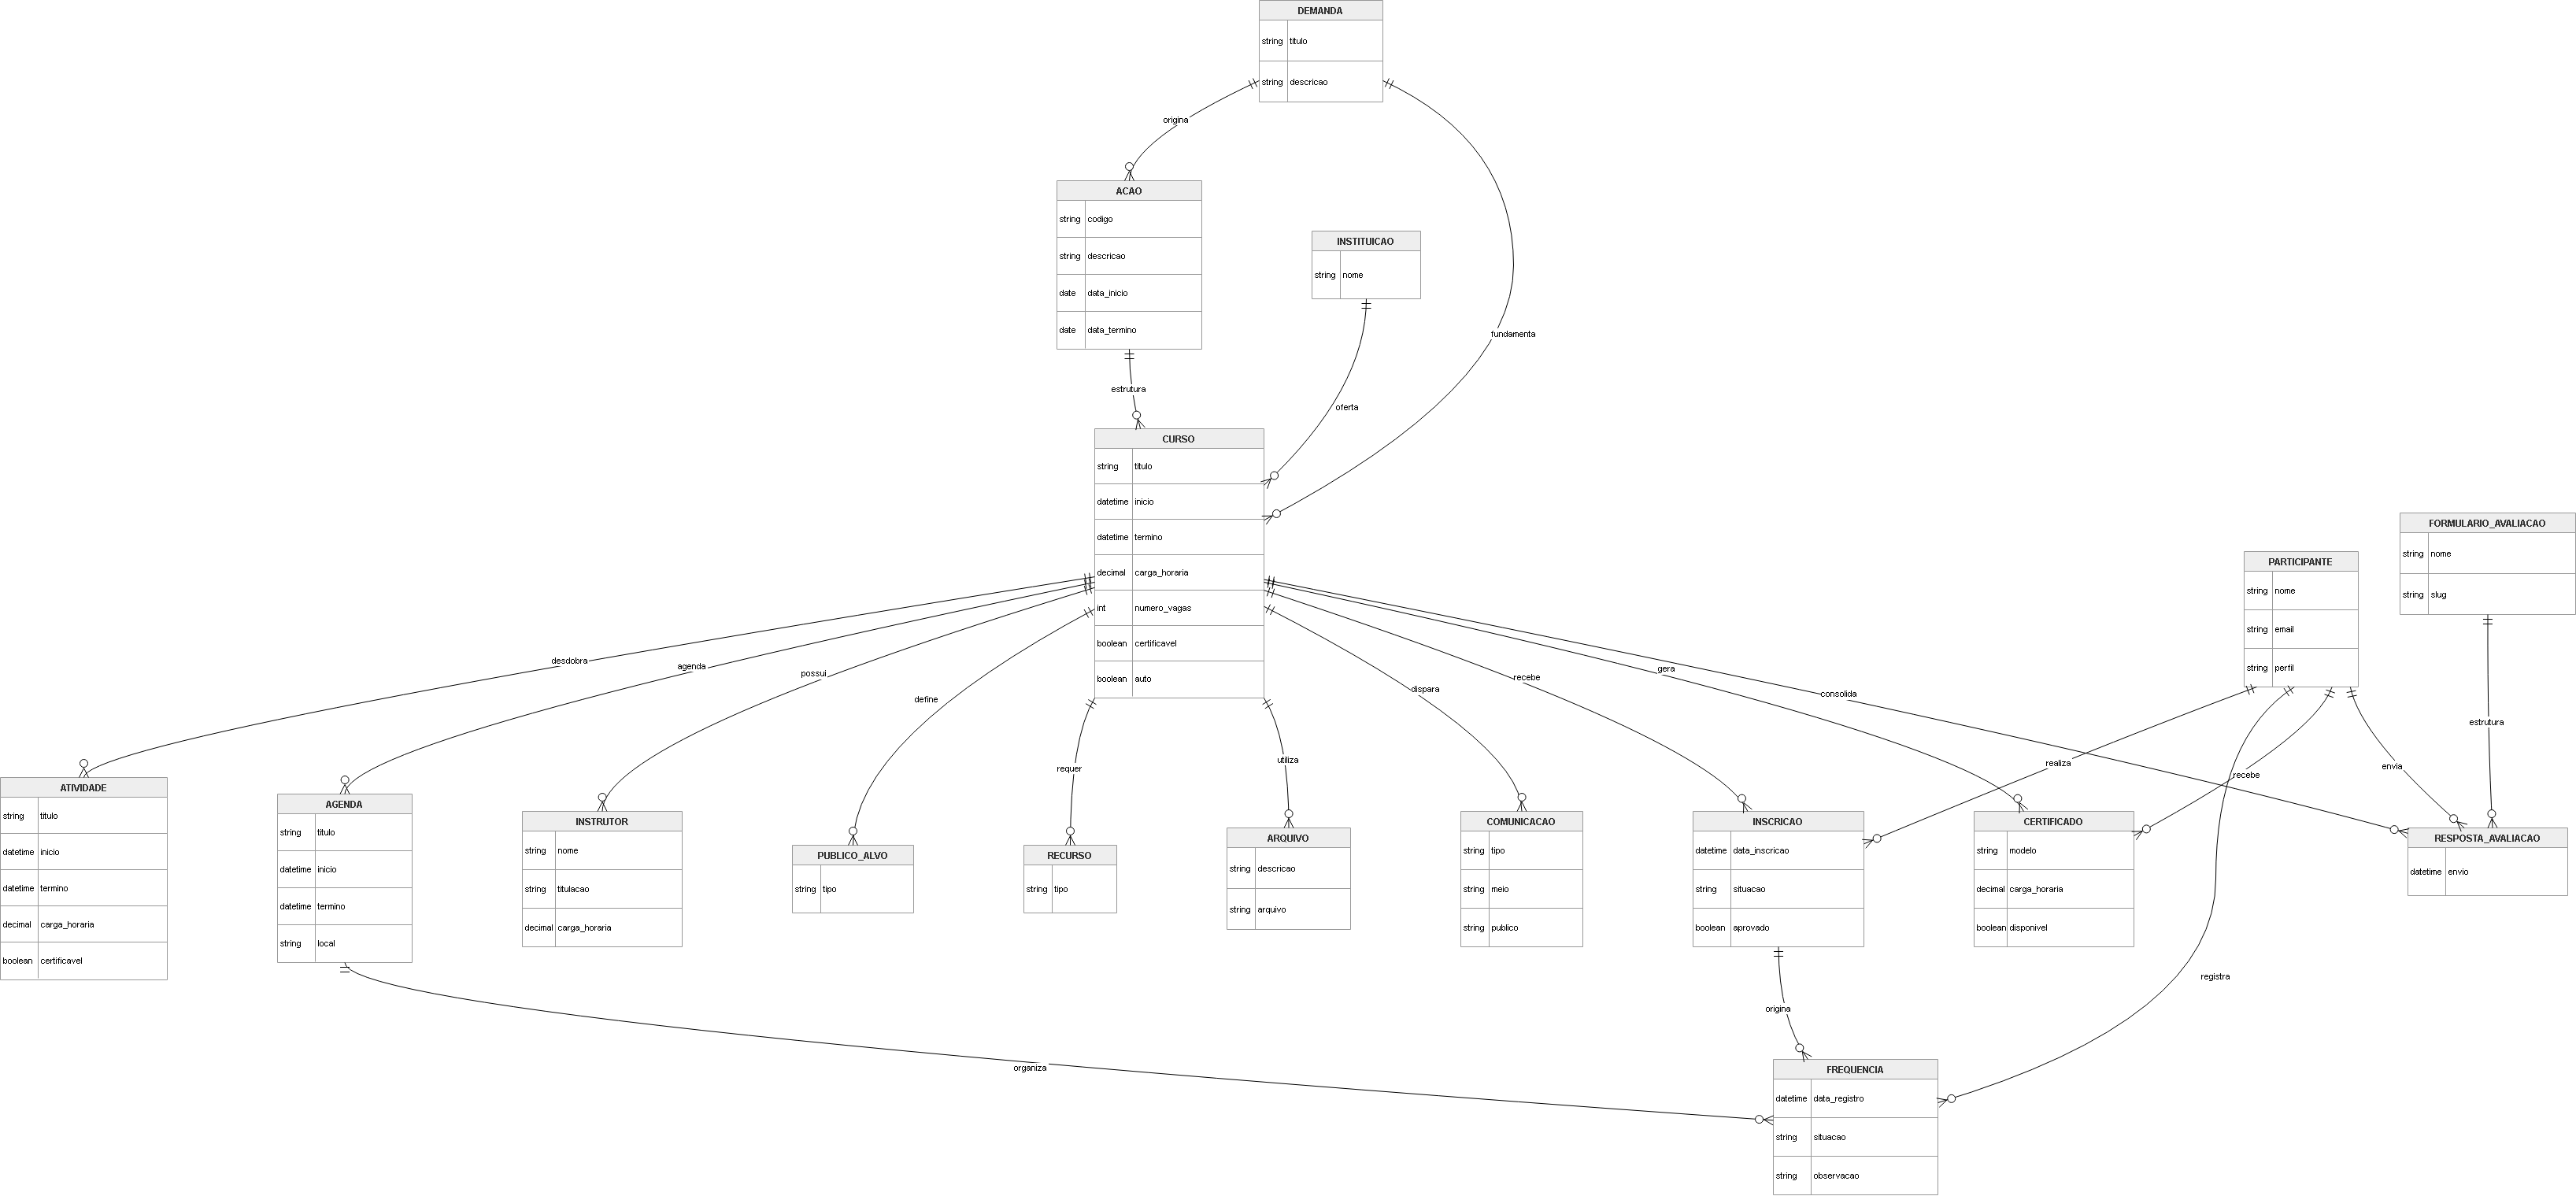
\includegraphics[width=\textwidth,height=0.82\textheight,keepaspectratio]{imagens/modelo-conceitual.png}
\end{center}

\noindent\textbf{Arquivo-fonte:} \texttt{imagens/modelo-conceitual.svg}

\section{Fluxo pedagógico conceitual}
\label{apend:diagramas-analise-sistema:fluxo-pedagogico}

Resume o encadeamento conceitual dos dados e das etapas que estruturam o
ciclo pedagógico observado no sistema.

\begin{center}
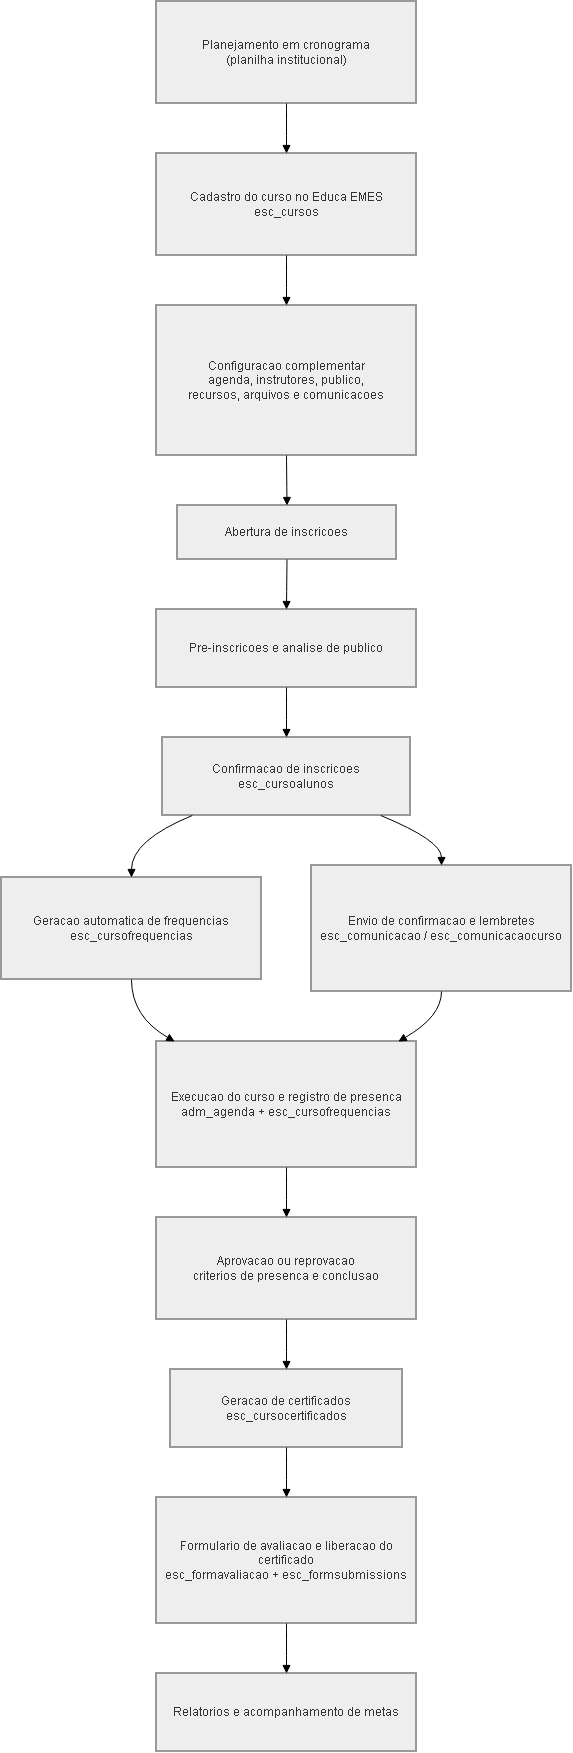
\includegraphics[width=\textwidth,height=0.82\textheight,keepaspectratio]{imagens/fluxo-pedagogico.png}
\end{center}

\noindent\textbf{Arquivo-fonte:} \texttt{imagens/fluxo-pedagogico.svg}
